\documentclass[10pt,a4paper]{article}
\usepackage{amsmath}
\usepackage{amsfonts}
\usepackage{amssymb}
\usepackage{natbib}
\usepackage{graphicx}
\usepackage[left=2cm,right=2cm,top=2cm,bottom=2cm]{geometry}
\usepackage{arydshln}
\usepackage{bm}
\title{Revealing Transient Strain in Geodetic Data with the Radial Basis Function Finite Difference Method}
\author{Trever T. Hines and Eric A. Hetland}

% OUTLINE
% INTRODUCTION
% - Why we care about strain in the crust
%   - Knowing long term strain rates tells us where we can expect seismicity
%
% - How people have gone about estimating strain rates
%   - Draw distinction between parametric and nonparametric methods
%   - Draw distinction between model based and data based parametric methods 
%   - Talk about Kato
%
% - Another, more challenging problem is how to calculate time-dependent strain
%   - Time dependent strain rates could illuminate transient geophysical signals such as postseismic deformation, 
%	  slow slip events, or volcanic deformation. 	  
%	- Since numerous megathrust earthquakes were preceded by slow slip, it is important to detect these features.
%	- We can also use estimates of transient strain to calibrate strain meters.	
%	- People who have tackled this problem before include Ohtani and Holt.	
%	- A major deficiency with these methods is that they are parametric giving poor uncertainties. Without good 
%	  uncertainties we cannot objectively discern signal from noise and we cannot calibrate BSM.	
% - Here we propose GPR and we tackle several two major difficulties	
%   - The method is similar to an extension of Kato to the time domain. We address two debilitating difficulties that 
%     arise. We also dont do that autocovariance bullshit.  Instead we use REML.  
%	- outliers  
%	- dense matrix
%	
% - GPR can be used for more than just estimating strain and it is a powerful geophysical tool. We can use it to quantify
%   spatial noise in GPS data. (this should be a side blurb when talking about quantifying signal.   
%
% - We discuss the method, form prior with REML, and demonstrate utility in detecting SSE by comparing it to tremor.	  
%
% METHODS
% - define model
% - discuss known deficiencies with the model
% - describe covariance as a time-space separable function 
% - describe geophysically relevant gaussian processes. (include seasonal and spherical)
% - REML for determining optimal hyperparameters
% - conditioning the prior with observations
% - differentiating the Gaussian process
% - note on addition, subtraction, and scaling
% - REML
% - Numerical notes
%   - partition inverse and solve with CHOLMOD
% - outlier detection

% APPLICATION TO CASCADIA SSE
% - SSE background
% - REML results
%   - noise 
%   - signal for IBM, SE, and WEN
%   - Plot all covariances functions

% - Strain results
%   - map view plot
%   - time series plot

% CONCLUSION
% - future work
% - additional applications other than sse. Discuss potential use for noise modeling


\begin{document}

\maketitle


\section{Introduction}\label{sec:Introduction}

Crustal strain rates are fundamentally important quantities for assessing seismic hazard, since knowing where and how quickly strain is accumulating gives insight into where we can expect stored elastic energy to be released seismically.  It is then important to develop and improve upon methods for mapping strain in tectonically active regions because such maps could conceivably feed into seismic hazard models such as UCERF3 \citep{Field2014}. 

Methods for estimating strain from geodetic data fall in one of two categories.  There are model-based approaches which assume that strain is the result of loading on faults which have a known geometry, and there are data-based approaches which make no assumptions about the source of deformation.  We will exclusively consider data-based approaches in this paper.  The classic and simplest method for estimating strain is to assume that the strain rate is constant in time and spatially uniform within subnetworks of the geodetic data.  Linear least squares is then used to find the components of the strain rate tensor for each subnetwork \citep[e.g][]{Frank1966,Prescott1976,Savage1986,Feigl1990,Murray2000}. Several algorithms have been developed to improve upon this procedure. \citet{Shen1996} and \citet{Shen2015} discuss an algorithm where, instead of using the immediately adjacent stations to calculate strain at a position, the strain is computed with a weighted average over the entire network where the weighting is smaller for more distant stations.  Another strategy is to fit a set of interpolating basis functions to the deformation field and then compute the strain from the analytical derivative of the interpolant \citep[e.g.][]{Beavan2001,Tape2009,Sandwell2016}.  

The aforementioned studies have all been concerned with estimating long term strain rates. Time dependent strain would be useful for studying geophysical processes which occur over timescales of days to years such as slow slip events, postseismic relaxation, or volcanic deformation.  \citet{Ohtani2010} identified transient strain events by fitting a set of spatial wavelet basis functions to the deformation field at discrete time epochs, and a Kalman filtering strategy was used to ensure that the coefficients for each basis function varied smoothly in time. \citet{Holt2013} calculated time dependent strain by differentiating a bicubic interpolant that was fit to each epoch of a temporally smoothed deformation field. 

Each of the methods described above are designed to overcome two complications that arise in estimating deformation gradients: (1) geodetic data are noisy and differentiation will only amplify the noise and (2) geodetic data are not observed on a regular grid, which prevents the use of standard finite difference methods for computing derivatives. In this paper we demonstrate that both of these complications can be elegantly handled with the Radial Basis Function-Finite Difference (RBF-FD) method.  

The RBF-FD method was developed simultaneously and independently by \citet{Tolstykh2003}, \citet{Shu2003}, \citet{Cecil2004}, and \citet{Wright2006} as a computationally efficient way to solve large scale partial differential equations over irregular, multi-dimensional domains.  The RBF-FD method can be thought of as a generalization of the traditional finite difference method, where the node layout is no longer restricted to regular grids. Indeed, the RBF-FD method can be used to estimate derivates of discrete data located at arbitrary scattered positions in multi-dimensional space.  The RBF-FD method is particularly appealing because it is algorithmically simple, regardless of the domain shape or node layout, and also because the method has performed well in numerous benchmark tests \citep[and references therein]{Fornberg2015}.

In this paper, we do not use the RBF-FD method to solve a partial differential equation, but rather we use it to spatially smooth geodetic data and to compute deformation gradients. Our smoothing strategy can be viewed as a non-parametric, low-pass filter for scattered data where the degree of smoothness is controlled by a user specifies cutoff frequency. This can be contrasted with interpolation based methods where the resulting interpolant can be largely and perhaps unpredictably controlled by the choice of basis function. This process of smoothing and differentiating can be extended to estimate time dependent strain rates.  In that case, we first temporally smooth and differentiate GPS displacement time series to get time dependent velocities.  We then spatially smooth and differentiate the resulting velocities for each time epoch to get time dependent strain rates.  

The method proposed in this paper has numerous advantages which set it apart from other methods for computing strain rates. The method is computationally efficient and stable (there is no inversion of an ill-conditioned matrix).  There are no hyper parameters or penalty parameters that need to be tuned for each application.  As opposed to interpolation strategies such as \citet{Beavan2001}, \citet{Tape2009}, or \citet{Ohtani2010}, our method assumes that velocities are locally rather than globally continuous, which allows us to easily handle discontinuities resulting from, for example, a creeping fault. 

We begin this paper by summarizing the RBF-FD scheme and explaining how we construct differentiation matrices for scattered data. We then introduce the RBF-FD filter, which is used to smooth the observed geodetic data prior to differentiation.  We provide two real world demonstraitions of our method for calculating strain rates.  First we calculate the long term strain rates in Southern California from the CMM3 velocity data set \citep{Shen2011}, and we verify that our results are consistent with other studies. We then calculate time dependent strain rates in Cascadia from the GPS data provided by UNAVCO.  In Cascadia, we analyze strain resulting from slow slip events and compare it to the long term tectonic strain accumulation. Slow slip events are found to produce compression in the Olympic Peninsula, which is in addition to the compression resulting from tectonic loading.  Further south in Oregon, the slow slip events tend to release the compressional strain that is accumulated tectonically.  While similar conclusions have been drawn from fault slip inversions for slow slip events, it is important to recognize that slip inversion are the product of inverting an ill-conditioned matrix making it difficult to determine whether slip inferences are real or just an artifact of the inversion.  The strain rates presented in this paper are more direct observations and can be interpretted with a higher degree of confidence. 

\section{Method}\label{sec:Method}
In this section, we describe how GNSS displacement observations are used to identify transient crustal strain rates, which we denote as $\dot{\bm{\varepsilon}}(z)$, where $z$ is the ordered pair $(x,t)$, $x$ are spatial coordinates in $\mathbb{R}^2$, and $t$ is time. We consider $\dot{\bm{\varepsilon}}$ to be spatially and temporally coherent deviations from the steady rate of strain accumulation from plate tectonics. We determine $\dot{\bm{\varepsilon}}$ by first identifying transient displacements, $\bm{u}(z)$, which we then spatially and temporally differentiate.  As we will show in Section X, estimates of $\dot{\bm{\varepsilon}}$ turn out to be more effective at illuminating geophysical signal than estimates of $\bm{u}$ or $\dot{\bm{u}}$.  We make a prior assumption that each component of $\bm{u}$ is a Gaussian process,
\begin{equation}\label{eq:TransientDeformation}
u_i(z) \sim \mathcal{N}\left(0,C_{u_i}\right),
\end{equation}
where $C_{u_i}(z,z')$ is a covariance function indicating how we expect $u_i(z)$ to covary with $u_i(z')$. For simplicity, we treat each component of displacement independently and ignore any potential covariance. We then drop the component subscripts with the understanding that the same analysis is being repeated to estimate the east, north, and vertical components of $\bm{u}$. We further assume that $C_u$ can be separated into positive definite spatial and temporal functions as 
\begin{equation}\label{eq:TransientCovariance}
C_{u}\left((x,t),(x',t')\right) = X(x,x')T(t,t'),
\end{equation}  
The appropriate choice for $X$ and $T$ may vary depending on the geophysical signal we are trying to describe (e.g. postseismic deformation or deformation from slow slip events), and we discuss this matter in the next section.  

We constrain $u$ with GNSS data, which records $u$ as well as other physical and non-physical processes which we are not interested in. We describe GNSS observations at position $x_i$ and time $t_j$ as a realization of the random variable 
\begin{align}\label{eq:Data}
\begin{split}
d_{ij} = &u(x_i,t_j) + \epsilon(x_i,t_j) + w_{ij} + a^{(1)}_i + a^{(2)}_it_j + \\
         &a^{(3)}_i\sin(2 \pi t_j) + a^{(4)}_i\cos(2 \pi t_j) + a^{(5)}_i\sin(4 \pi t_j) + a^{(6)}_i\cos(4 \pi t_j), 
\end{split}
\end{align}
where $a^{(1)}_{i}$ is an offset that is unique for each GNSS monument, $a^{(2)}_{i}$ is the steady rate of tectonic deformation at $x_i$, and the sinusoids describe seasonal deformation (using units of years for $t$). We use $w_{ij}$ to denote normally distributed, uncorrelated noise. Correlated noise which does not have a parametric representation is denoted by $\epsilon$.  For example, $\epsilon$ can consist of temporally correlated noise describing benchmark wobble \citep[e.g.,][]{Wyatt1982,Wyatt1989}, and/or spatially correlated noise describing common mode error \citep[e.g.,][]{Wdowinski1997}. For now, we will only assume that $\epsilon \sim \mathcal{N}(0,C_\epsilon)$. We consider the six coefficients in eq. (\ref{eq:Data}) to be uncorrelated random variables distributed as $\mathcal{N}(0,\kappa^2)$ in the limit as $\kappa \to \infty$ (i.e., the coefficients have diffuse priors). Of course, the tectonic deformation, $a^{(2)}_{i}$, is spatially correlated and we could invoke a tectonic model to form a prior on $a^{(2)}_{i}$. However, in our application to Cascadia, we will be using displacement time series which are long enough to sufficiently constrain $a^{(2)}_{i}$ for each station, and there is no need to incorporate a prior. Likewise, the seasonal coefficients may be spatially correlated \citep{Langbein2008}, and it may be worth exploring and exploiting such a correlation in a future study. 

We now consider the column vector of $n$ GNSS observations, $\bm{d}_*$. Let $\bm{y}$ be the set of $(x_i, t_j)$ pairs describing where and when each of the GNSS observations have been made. Let $\bm{a}$ be the vector of coefficients from eq. (\ref{eq:Data}) for each of the $m$ GNSS stations. We use $\bm{P}$ to represent the $n \times 6m$ matrix of corresponding basis functions evaluated at each point in $\bm{y}$. We  also denote the vector of uncorrelated noise for each observation as $\bm{w}$, whose standard deviations are given by the formal data uncertainty $\bm{\sigma}$. The observations $\bm{d}_*$ can then be viewed as a realization of the random vector
\begin{equation}
\bm{d} = u(\bm{y}) + \epsilon(\bm{y}) + \bm{w} + \bm{P}\bm{a},
\end{equation}
which is distributed as $\mathcal{N}(\bm{0},\bm{\Sigma} + \kappa^2\bm{P}\bm{P}^T)$, where
\begin{equation}\label{eq:Cd}
\bm{\Sigma} = C_u(\bm{y},\bm{y}) + C_\epsilon(\bm{y},\bm{y}) + 
              \mathrm{diag}\left(\bm{\sigma}^2\right).  
\end{equation}
It should be understood that the notation $f(\bm{x})$ and $f(\bm{x},\bm{y})$ is shorthand for $[f(x_i)]_{x_i \in \bm{x}}$ and $[f(x_i,y_j)]_{(x_i,y_j) \in \bm{x} \times \bm{y}}$, respectively. 

We now describe how to condition the prior for each component of transient displacements, $u$, with $\bm{d}_*$ to form a posterior estimate of transient displacements, $\hat{u} = u | \bm{d}_*$. We will assume that an appropriate covariance functions and corresponding hyperparameters for $X$, $T$, and $C_\epsilon$ have already been chosen. If $\kappa$ is kept finite, then we can follow \citet{Rasmussen2006} to find that $\hat{u}$ is distributed as $\mathcal{N}(\mu_{\hat{u}},C_{\hat{u}})$, where
\begin{equation}\label{eq:PosteriorMean}
\mu_{\hat{u}}(z) = C_u(z,\bm{y})\left(\bm{\Sigma} + \kappa^2\bm{P}\bm{P}^T\right)^{-1}\bm{d}_*
\end{equation}    
and
\begin{equation}\label{eq:PosteriorCov}
C_{\hat{u}}(z,z') = C_u(z,z') - C_u(z,\bm{y})\left(\bm{\Sigma} + \kappa^2\bm{P}\bm{P}^T\right)^{-1}C_u(\bm{y},z').
\end{equation}
However, we are interested in the limit as $\kappa \to \infty$, and the form for eq. (\ref{eq:PosteriorMean}) and eq. (\ref{eq:PosteriorCov}) is not suitable for evaluating this limit. We can use the partitioned matrix inversion identity \citep[e.g.,][]{Press2007} to rewrite eq. (\ref{eq:PosteriorMean}) and eq. (\ref{eq:PosteriorCov}) as
 \begin{equation}\label{eq:PosteriorMean2}
\mu_{\hat{u}}(z) =
\left[ 
\begin{array}{cc}
C_u(z,\bm{y}) & \bm{0} \\
\end{array}
\right]
\left[
\begin{array}{cc}
\bm{\Sigma} & \bm{P} \\
\bm{P}^T  & -\kappa^{-2} \bm{I} \\
\end{array}
\right]^{-1}
\left[
\begin{array}{c}
\bm{d}_* \\
\bm{0} \\
\end{array}
\right]
\end{equation}    
and
\begin{equation}\label{eq:PosteriorCov2}
C_{\hat{u}}(z,z') = 
C_u(z,z') - 
\left[ 
\begin{array}{cc}
C_u(z,\bm{y}) & \bm{0} \\
\end{array}
\right]
\left[
\begin{array}{cc}
\bm{\Sigma} & \bm{P} \\
\bm{P}^T  & -\kappa^{-2} \bm{I} \\
\end{array}
\right]^{-1}
\left[
\begin{array}{c}
C_u(\bm{y},z') \\
\bm{0} \\
\end{array}
\right].
\end{equation}
Taking the limit as $\kappa \to \infty$, we get the solution for the mean and covariance of $\hat{u}$,
 \begin{equation}\label{eq:PosteriorMean3}
\mu_{\hat{u}}(z) =
\left[ 
\begin{array}{cc}
C_u(z,\bm{y}) & \bm{0} \\
\end{array}
\right]
\left[
\begin{array}{cc}
\bm{\Sigma} & \bm{P} \\
\bm{P}^T  & \bm{0} \\
\end{array}
\right]^{-1}
\left[
\begin{array}{c}
\bm{d}_* \\
\bm{0} \\
\end{array}
\right]
\end{equation}    
and
\begin{equation}\label{eq:PosteriorCov3}
C_{\hat{u}}(z,z') = 
C_u(z,z') - 
\left[ 
\begin{array}{cc}
C_u(z,\bm{y}) & \bm{0} \\
\end{array}
\right]
\left[
\begin{array}{cc}
\bm{\Sigma} & \bm{P} \\
\bm{P}^T  & \bm{0} \\
\end{array}
\right]^{-1}
\left[
\begin{array}{c}
C_u(\bm{y},z') \\
\bm{0} \\
\end{array}
\right].
\end{equation}

The posterior transients displacements, $\hat{\bm{u}}$, are found by evaluating eq. (\ref{eq:PosteriorMean3}) and (\ref{eq:PosteriorCov3}) for each displacement component. We differentiate the Gaussian process $\hat{\bm{u}}$ (see \cite{Abrahamsen1997}) to form an estimate of transient strain rate, $\dot{\bm{\epsilon}}$, which is itself a spatially and temporally continuous Gaussian process. The components of the transient strain rate tensor, $\dot{\epsilon}_{ij}$, are given by
\begin{equation}\label{eq:StrainRate}
\dot{\epsilon}_{ij}(z) = \frac{1}{2} \frac{\partial}{\partial t} \left(
                                     \frac{\partial \hat{u}_i(z)}{\partial x_j} +  
                                     \frac{\partial \hat{u}_j(z)}{\partial x_i}\right).
\end{equation}
which are distributed as $\mathcal{N}(\mu_{\dot{\epsilon}_{ij}},C_{\dot{\epsilon}_{ij}})$, where
\begin{equation}\label{eq:StrainMean}
\mu_{\dot{\epsilon}_{ij}}(z) = \frac{1}{2}\frac{\partial}{\partial t}\left(
                               \frac{\partial \mu_{\hat{u}_i}(z)}{\partial x_j} + 
                               \frac{\partial \mu_{\hat{u}_j}(z)}{\partial x_i} \right)
\end{equation} 
and  
\begin{equation}\label{eq:StrainCov}
C_{\dot{\epsilon}_{ij}}(z,z') = \frac{1}{4} \frac{\partial^2}{\partial t \, \partial t'}\left(
                           \frac{\partial^2 C_{\hat{u}_i}(z,z')}{\partial x_j \, \partial x'_j} + 
                           \frac{\partial^2 C_{\hat{u}_j}(z,z')}{\partial x_i \, \partial x'_i} \right).
\end{equation} 

\subsection{Outlier detection}\label{sec:Outlier}
In our formulation for estimating transient strain rates, we have assumed that noise in the data vector is normally distributed. This is not an appropriate assumption for GNSS displacement timeseries which are prone to more outliers than would be predicted for normally distributed noise. It follows that proposed methods for analyzing GNSS timeseries should be robust against outliers \citep[e.g.,][]{Blewitt2016}. In order to make our estimates of transient strain more robust, we automatically identify and remove outliers in the GNSS data as a pre-processing step.

Our method for detecting outliers is based on the data editing algorithm described in \citet{Gibbs2011}. We calculate the residuals between the observations and a best fitting model, and data with residuals that are anomalously large are identified as outliers. We treat $\bm{d}_*$ as a sample of $\bm{d}$ and assume that there is no temporally correlated noise (i.e., $\epsilon = 0$).  The best fitting model for $\bm{d}_*$ is considered to be the expected value of the random vector $u(\bm{y}) + \bm{P}\bm{a}$ after conditioning it with non-outlier observations.  We still consider $u$ to have a separable covariance function as in eq. (\ref{eq:TransientCovariance}), and the choice for $X$ and $T$ does not need to be the same as that used in Section X. Since outliers are determined based on how well a spatially and temporally dependent model fits the data, we are able to identify anomalous observations which may not be immediately apparent based on inspection of individual timeseries. 

To begin the algorithm, we let $\Omega$ be the index set of non-outliers in $\bm{d}_*$ and initiate it with all $n$ indices. This algorithm is iterative, and for each iteration we calculate the residual vector
\begin{align}\label{eq:Residual}
\bm{r} &= \frac{\bm{d}_* - \mathrm{E}\left[(u(\bm{y}) + \bm{P}\bm{a})|\tilde{\bm{d}}_* \right]}{\bm{\sigma}} \\
       &= \frac{1}{\bm{\sigma}}\left(\bm{d}_*  - 
\left[ 
\begin{array}{cc}
C_u(\bm{y},\tilde{\bm{y}}) & \bm{P} \\
\end{array}
\right]
\left[
\begin{array}{cc}
C_u(\tilde{\bm{y}},\tilde{\bm{y}}) + \mathrm{diag}(\tilde{\bm{\sigma}}^2) & \tilde{\bm{P}} \\
\tilde{\bm{P}}^T  & \bm{0} \\
\end{array}
\right]^{-1}
\left[
\begin{array}{c}
\tilde{\bm{d}}_* \\
\bm{0} \\
\end{array}
\right] 
\right),
\end{align}
where the tilde indicates that only elements corresponding to indices in $\Omega$ are retained (e.g., $\tilde{\bm{y}} = \{y_i\}_{i\in\Omega}$). We then update $\Omega$ to be
\begin{equation}\label{eq:Update}
\Omega = \{i : |r_i| < \eta \tilde{\bm{r}}_{rms}\}, \ \ \ r_i \in \bm{r}
\end{equation} 
where $\tilde{\bm{r}}_{rms}$ is the root-mean-square of $\tilde{\bm{r}}$ and $\eta$ is an outlier tolerance. We use $\eta=4$ in this study, which seems to accurately identify outliers without unnecessarily decimating the data. Iterations continue until the new $\Omega$ is equal to the previous $\Omega$. 

It should be noted that this algorithm does not identify jumps in GNSS time series, which are another common defect. Some, but not all, jumps can be automatically removed by parsing station logs and identifying dates of antenna changes. However, it is still necessary to manually inspect and remove jumps of unknown origin. That being said, this outlier detection algorithm significantly reduces the effort needed to manually clean GNSS data.       

\section{Application Cascadia Slow Slip Events}\label{sec:Cascadia}
In this section we estimate transient strain from GNSS data in Cascadia. We are mainly interested in identifying transient strain resulting from slow slip events (SSEs) \citep[e.g.,][]{Dragert2001}. We show that Gaussian processes are an effective tool for (1) detecting SSEs and (2) understanding how the strain from SSEs are contributing to the strain accumulated over the seismic cycle. Our motivation for detecting SSEs is, in part, because there have been several instances where SSEs immediately preceded megathrust earthquakes \citep{Roeloffs2006}.  In Cascadia, SSEs can be detected by monitoring for associated seismic tremor, which is actively being done by the Pacific Northwest Seismic Network (PNSN) \citep{Wech2010}. 
Here we demonstrate that strain rates derived from GNSS data can also be an effective tool for detecting SSEs. Furthermore, estimated strain rates provide a clear picture of how SSEs transfer elastic strain energy through the crust, which is also important information for assessing seismic hazard. We envision that GNSS derived transient strain rates could be useful for monitoring subduction zones which have SSEs but no associated tremor \citep{Schwartz2007}.

In this study, we use GNSS data which has been made publicly available by the University Navstar Consortium (UNAVCO) \citep{Herring2016} and can be found at www.unavco.org.  We limit the dataset to the stations and time ranges which are pertinent to seven of the most recent SSEs in the Puget Sound region; the earliest SSE began in the August 2010, and the most recent SSE began in the February of 2017. We consider these most recent SSEs because the station coverage is sufficiently dense for us to make well constrained inferences of optimal prior models.  The distribution of stations considered in this station is shown in Figure X. 


\subsection{Noise model}\label{sec:NoiseModel}
In this section we discuss our choice for the noise covariance function $C_\epsilon$ which will be used when estimating transient strain.  There have been numerous studies on temporally correlated noise in GNSS data \citep[e.g.,][]{Zhang1997,Mao1999,Williams2004,Langbein2008}. In these studies, temporally correlated noise was described with some combination of Brownian motion, first-order Gauss-Markov (FOGM) processes, and/or flicker noise. There is some physical justification for using Brownian motion as a noise model because it accurately describes the power spectrum of motion resulting from instability in geodetic monuments \citep[e.g.,][]{Wyatt1982,Wyatt1989,Langbein1997}. Here we describe the time dependence of $\epsilon$ as a FOGM process and consider $\epsilon$ to be spatially uncorrelated. A FOGM process is a solution to the stochastic differential equation
\begin{equation}
\dot{\epsilon}(t) + \alpha \epsilon(t) = \beta w(t),
\end{equation}
where $w(t)$ is white noise with unit variance. The noise model is then a Gaussian process with zero mean and covariance function
\begin{equation}\label{eq:FOGM}
C_\epsilon\left((x,t),(x',t')\right) = \frac{\beta^2}{2\alpha}\exp\left(-\alpha|t - t'|\right) \delta(||x - x'||_2). 
\end{equation}
Under the condition that $\alpha = 0$ and $v(0) = 0$, $\epsilon$ degenerates to the more commonly used Brownian motion noise model. 

We constrain the hyperparameters for $\epsilon$, $\alpha$ and $\beta$, with a set of 38 inland stations, which are shown in Figure X. These stations are sufficiently far from the subduction zone that they are unlikely to contain transient signal. We clean the data for these stations by removing jumps at times of equipment changes, and we remove outliers that have been detected with the algorithm described in Section \ref{sec:Outlier}. We then find $\alpha$ and $\beta$ for each station timeseries with the Restricted Maximum Likelihood (REML) method \cite[e.g.,][]{Harville1974,Cressie1992} and Hines 2017. The REML method finds the hyperparameters which maximize the expression
\begin{equation}\label{eq:REML}
\left(\frac{\left|\bm{P}^T\bm{P}\right|}
           {(2\pi)^{n-6m}
            \left| \bm{\Sigma} \right| 
            \left| \bm{P}^T\bm{\Sigma}\bm{P} \right|}\right)^{\frac{1}{2}} 
e^{-\tfrac{1}{2}\bm{d}_*^T\bm{K}\bm{d}_*},
\end{equation}
where
\begin{equation}
\bm{K} = \bm{\Sigma}^{-1} - 
         \bm{\Sigma}^{-1}\bm{P}
         \left(\bm{P}^T\bm{\Sigma}^{-1}\bm{P}\right)^{-1}
         \bm{P}^T\bm{\Sigma}^{-1}.
\end{equation}
For this section, $\bm{d}_*$ is used to denote the displacement time series for just one station, and thus $m = 1$. We are also assuming $C_u$ is zero when estimating the noise hyperparameters for this section. \citet{Harville1974} showed that choosing the hyperparameters which maximize eq. (\ref{eq:REML}) is equivalent to chosing the hyperparameters which maximize the probability of drawing $\bm{d}_*$ from $\bm{d}$.  We use the REML method over the maximum likelihood (ML) method \citep[e.g.,][]{Langbein1997} because the REML method properly accounts for the improper prior that we assigned to $\bm{a}$. The distribution of inferred $\alpha$ and $\beta$ are shown in Figure \ref{fig:NoiseParams}. The amplitude of FOGM noise for the east and north components is notable low and are clustered around 0.5 mm/yr$^{0.5}$. The corresponding estimates of $\alpha$ tend to cluster around 0 yr$^{-1}$, suggesting that Brownian motion would have also been an appropriate noise model.  The amplitude of FOGM noise for the vertical component is significantly larger with a median value of 13.8 mm/yr$^{0.5}$. The inferred values for alpha are higher for the vertical component with a median value of 1.87 yr$^{-1}$. In Figure X, we use the median values of $\alpha$ and $\beta$ to generate two random samples of FOGM noise. The samples span seven years and over these seven years the east and north samples drift by about 1 mm. In the context of detecting SSEs, which produce several mm's of surface displacement on the timescale of weeks, the estimated FOGM noise for the east and north component is negligible. In contrast, the estimated FOGM noise for the vertical component is significantly larger than the signal we would expect from SSEs. We suspect that the higher amplitude for the FOGM model in the vertical component is accommodating for deficiencies in our rather simple seasonal model. Based on this analysis, we henceforth ignore temporally correlated noise in the east and north component because of its low amplitude, and we do not estimate $u$ for vertical deformation because of the low signal to noise ratio.

\begin{figure*}
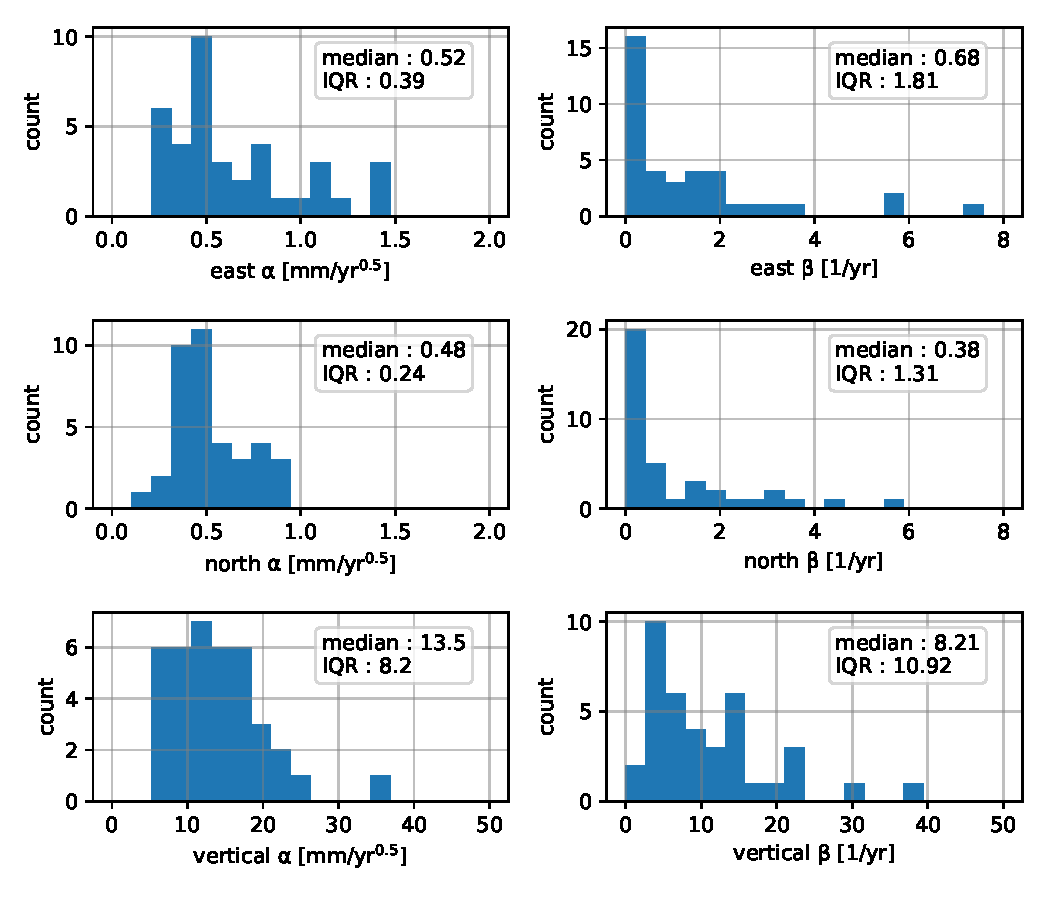
\includegraphics{figures/noise/noise-params.pdf}
\caption{Distribution of estimated FOGM hyperparameters from eq. (\ref{eq:FOGM}).  Hyperparameters are independently estimated for each of the stations shown in Figure X and for each displacement component. ``IQR'' is the inter-quartile range.}   
\label{fig:NoiseParams}
\end{figure*}

\begin{figure*}
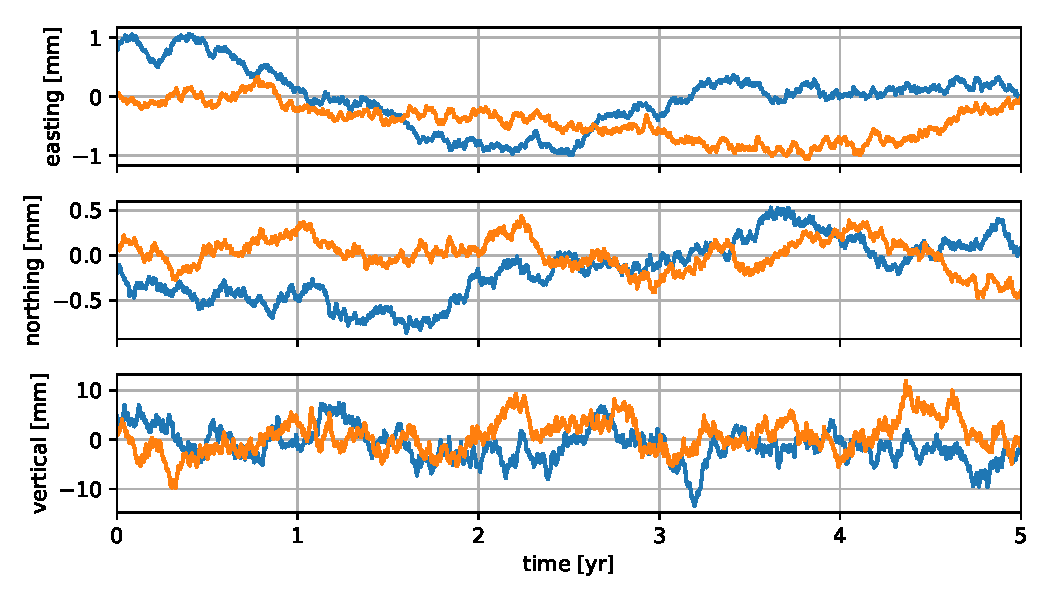
\includegraphics{figures/noise/noise-samples.pdf}
\caption{Two FOGM noise samples, where the hyperparameters have been set to the median values from Figure \ref{fig:NoiseParams}.}   
\label{fig:NoiseSamples}
\end{figure*}


Another significant source of noise in GNSS data is common mode error \citep[e.g.,][]{Wdowinski1997,Dong2006}, which is noise that is highly spatially correlated. When not accounted for, common mode error manifests itself as spatially uniform undulations in $\hat{u}$. However, we are primarily interested in estimating strain which is insensitive to common mode error. We therefore do not include common mode error in our noise model. 

For these reasons, we henceforth make the simplifying assumption that temporally and spatially correlated noise is negligible and $\epsilon = 0$ for the easting and northing component of GNSS data.            

\subsection{Transient displacement model}\label{sec:SignalModel}
We next discuss our prior model for transient displacements, and, specifically, our choice for the covariance functions $X(x,x')$ and $T(t,t')$. For $X$, we use the squared exponential (SE) covariance function,
\begin{equation}\label{eq:SE}
X(x,x') = \exp\left(\frac{-||x - x'||_2^2}{2 \lambda^2}\right).
\end{equation}
The SE covariance function is commonly used in Kriging \citep[e.g,][]{Cressie1992} and Gaussian process regression \citep[e.g.,][]{Rasmussen2006}.  The SE is a valid (i.e. positive definite) covariance function for any number of spatial dimensions, and it describes an isotropic Gaussian processes with realizations that are infinitely differentiable. In terms of geodetic applications, \citet{Kato1998} and \cite{El-Fiky1999} demonstrated that the SE is an appropriate covariance model for describing long-term tectonic strain rates in Japan.  

We consider three potential covariance functions to describe the temporal covariance of $u$.  First, we consider the one-dimensional SE covariance function, 
\begin{equation}\label{eq:TimeSE}
T(t,t') = \phi^2\exp\left(\frac{-|t - t'|^2}{\theta^2}\right),
\end{equation}
simply because the SE covariance function is versatile and commonly used for non-parametric modeling. Note that $T$ includes the hyperparameter $\phi$, which serves to scale the covariance function $C_u$. Second, we consider integrated Brownian motion (IBM). IBM has zero mean and its covariance function can be found by integrating the covariance function for Brownian motion as
\begin{align}\label{eq:IBM}
T(t,t') &= \int_0^t \int_0^{t'} \phi^2 \min(\tau,\tau') \,d\tau'\,d\tau \\
        &= \frac{\phi^2}{2}\min(t,t')^2 \left(\max(t,t') - \frac{1}{3}\min(t,t')\right), \ \ \ t,t' \geq 0.
\end{align}
IBM has been used, in the context of Kalman filtering, as a non-parametric model for the time dependence of geophysical signals \citep[e.g.,][]{Segall1997,McGuire2003,Ohtani2010,Hines2016}. It should be emphasized $t=0$ is a reference time at which the Gaussian process is exactly zero.  For some geophysical signals, it is appropriate to have this reference time. For example, if we are trying to identify postseismic deformation then $t$ should be zero at the time of the earthquake.  However, if we are interesting in detecting transient events, where there is no known start time, then IBM may not be an appropriate prior and an isotropic Gaussian process should be preferred. In the following analysis, we make the quite arbitrary choice that $t$ is zero on the first epoch of $\bm{d}_*$.  Our third option for $T$ is the Wendland class of covariance functions \citep{Wendland2005}. Wendland covariance functions have compact support and hence their corresponding covariance matrices will be sparse. In our analysis, we exploit this sparsity with the CHOLMOD software package \citep{Chen2008}.  Wendland functions are positive definite in $\mathbb{R}^d$, and they describes an isotropic Gaussian process with realizations that can be differentiated $k$ times. The form of the covariance function depends on the choice of $d$ and $k$. To describe the temporal covariance of $u$, we only require that $d=1$ and $k=1$. The corresponding Wendland covariance function is 
\begin{equation}\label{eq:Wendland}
T(t,t') = \phi^2\left(1 - \frac{|t - t'|}{\theta}\right)^3_+ \left(\frac{3|t - t'|}{\theta} + 1\right), 
\end{equation}
where
\begin{equation}
(t)_+ = 
\begin{cases}
t, \ \ \ t > 0 \\
0, \ \ \ \mathrm{otherwise}.
\end{cases}
\end{equation}

We next want to determine appropriate hyperparameters for $X$ and each of the three candidate functions for $T$. First, we again clean the GNSS datasets by removing offsets at times of equipment changes and removing outliers with the method describe in Section \ref{sec:Outlier}. For the outlier detection algorithm, our prior model, $u$, is chosen to have a length-scale and time-scale which is able to approximately describe SSE displacements. We use the SE covariance function for $X$ with $\lambda = 100$ km, and we use the Wendland covariance function for $T$, due to its computational efficiency, with $\theta = 0.1$ yr and $\phi = 1$ mm. The outlier detection algorithm is particularly effective at removing outliers for stations at high elevation, which can be adversely affected by ice or snow during the winter \citep{Lisowski2008}. As an example, Figure \ref{fig:Outliers} shows the outliers which were automatically detected for station SC03, which is located on Mount Olympus in Washington.  After cleaning the data, we divide it into subsets which are four months long and centered on the time of an SSE. The times of seven SSEs are determined using tremor records from \cite{Wech2010}. We find the optimal hyperparameters for $T$ and $X$ for each subset of data. The REML method is once again used to determine the hyperparameters for $T$ and $X$ which maximize the probability of drawing $\bm{d}_*$ from $\bm{d}$, where $\bm{d}_*$ now refers to a data subset. We chose to make each data subsets four months long because it is long enough to encompass the SSE, and it is short enough to still be computationally tractable. However, four months is too short to resolve the sinusoids in $\bm{d}$, and they are omitted from $\bm{d}$ for the REML analysis. The estimated hyperparameters for $u$ are summarized in Table 1. When using SE or the Wendland function for $T$, the optimal hyperparameters appear have a unimodal distribution. When using IBM for $T$ there were several anomalously large inferences, hence the larger IQR.   

\begin{figure*}
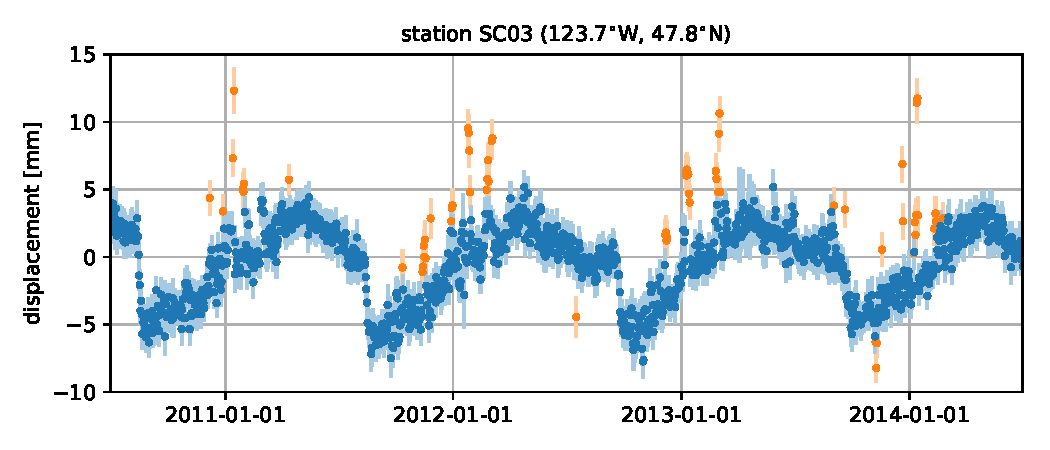
\includegraphics{figures/outliers/outliers.pdf}
\caption{Detrended easting component of GNSS displacement data for station SC03, which is located on Mt. Olympus in Washington.  The orange markers indicate outliers which were automatically detected using the algorithm from Section \ref{sec:Method}. The error bars show one standard deviation uncertainty.}   
\label{fig:Outliers}
\end{figure*}

\begin{table}\label{tab:Parameters}
\begin{tabular} {l l l l l l}
$T$ & direction & $\lambda$  & $\phi$   & $\theta$  & diff. $\log$(REML) \\ \hline
SE & east   & 92 $\pm$ 25 km  & 0.62 $\pm$ 0.11 mm  & 0.026 $\pm$ 0.011 yr  &  - \\
SE & north  & 91 $\pm$ 53 km  & 0.43 $\pm$ 0.05 mm  & 0.030 $\pm$ 0.017 yr  &  - \\
Wendland & east   & 95 $\pm$ 30 km  & 0.66 $\pm$ 0.15 mm  & 0.093 $\pm$ 0.044 yr &  0.78 $\pm$ 0.87 \\
Wendland & north  & 92 $\pm$ 57 km  & 0.46 $\pm$ 0.10 mm  & 0.116 $\pm$ 0.057 yr &  0.08 $\pm$ 0.58 \\
IBM & east   & 110 $\pm$ 130 km & 290 $\pm$ 420 mm/yr$^{1.5}$  & -          & -16.4 $\pm$ 7.8 \\
IBM & north  & 150 $\pm$ 560 km & 110 $\pm$ 250 mm/yr$^{1.5}$ & -           & -10.1 $\pm$ 2.3 \\
\end{tabular}
\caption{Hyperparameters. The shown values are the medians and interquartile ranges.} 
\end{table}


Next we identify which covariance function for $T$ best describes the SSEs. One approach is to compare the REML likelihood for each covariance function, similar to the analysis in \citet{Langbein2004}. In Table 1, we summarize how the log REML likelihoods for the Wendland and IBM covariance functions compare to the SE covariance function.  The tabulated values show the median and IQR differences in log REML likelihoods over each of the seven SSEs considered in this study. Negative values indicate that the observed data is less likely to have been sampled from the covariance function. Based on the differences in log REML likelihoods, the data is substantially more likely to come form the SE or Wendland covariance functions than from the IBM covariance function. The REML likelihoods do not definitively indicate whether the SE or Wendland covariance function is preferable. 

As another test to determine the most appropriate covariance function for $T$, we compare the observations to the predicted displacements for each covariance function. let $\hat{\bm{d}} = \left(u(\bm{y}) + \bm{P}\bm{a}\right)|\bm{d}_*$ be the data prediction vector. It can be shown that $\hat{\bm{d}}$ is normally distributed with mean 
\begin{equation}\label{eq:DataPredMean}
\bm{\mu}_{\hat{d}} =
\left[ 
\begin{array}{cc}
C_u(\bm{y},\bm{y}) & \bm{P} \\
\end{array}
\right]
\left[
\begin{array}{cc}
\bm{\Sigma} & \bm{P} \\
\bm{P}^T  & \bm{0} \\
\end{array}
\right]^{-1}
\left[
\begin{array}{c}
\bm{d}_* \\
\bm{0} \\
\end{array}
\right]
\end{equation}  
and covariance
\begin{equation}\label{eq:DataPredCov}
\bm{C}_{\hat{\bm{d}}} = 
C_u(\bm{y},\bm{y}) - 
\left[ 
\begin{array}{cc}
C_u(\bm{y},\bm{y}) & \bm{P} \\
\end{array}
\right]
\left[
\begin{array}{cc}
\bm{\Sigma} & \bm{P} \\
\bm{P}^T  & \bm{0} \\
\end{array}
\right]^{-1}
\left[
\begin{array}{c}
C_u(\bm{y},\bm{y}) \\
\bm{P}^T \\
\end{array}
\right].
\end{equation}
We compute $\hat{\bm{d}}$ using SE, Wendland, and IBM covariance functions for $T$ and the median hyperparameters from Table 1. Figure 1 compares the easting component of $\bm{d}_*$ to $\hat{\bm{d}}$ for the Winter 2016 SSE.  For most stations, the data prediction vector appears to appropriately describe displacements throughout the SSE, regardless of the choice of $T$. The prediction for the IBM model contains slightly more high frequency, and perhaps spurious, features. The predictions for the Wendland and SE covariance functions are nearly indistinguishable. We ultimately settle on the Wendland covariance function for $T$. We choose the Wendland covariance function over the SE covariance function because of its computational advantages noted above.     

\begin{figure*}
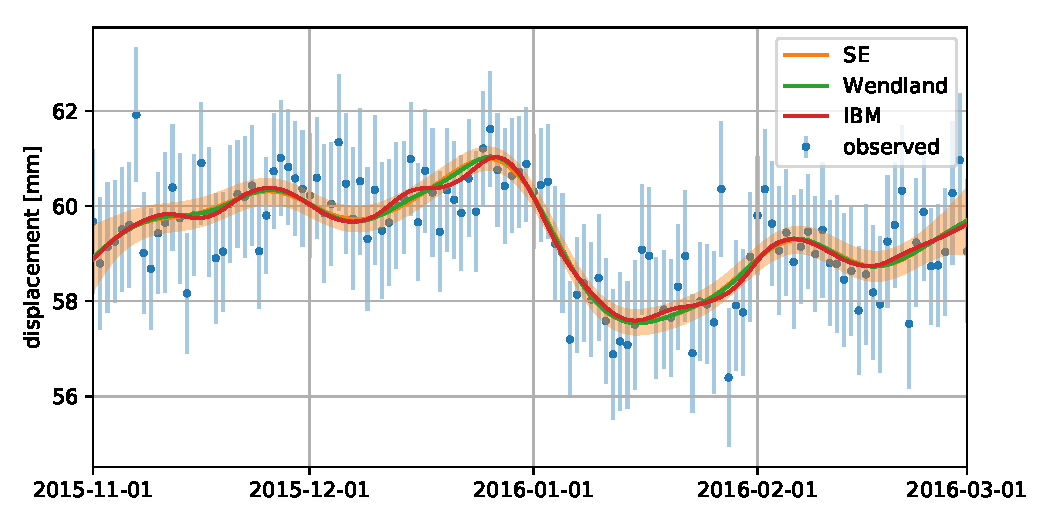
\includegraphics{figures/signal_fit/signal-fit.pdf}
\caption{Fit.}   
\label{fig:Fit}
\end{figure*}

\subsection{Transient Strain Rates} 
Having established noise model and a prior for transient displacements, we use cleaned GNSS dataset described in Section \ref{sec:SignalModel} to calculate transient strain rates in the Puget Sound region from eq. (\ref{eq:StrainRate}). Our solution is shown in Figures X through X. Figures X through X show the estimates $\dot{\bm{\epsilon}}$ complete with uncertainties at select times over the course of the Winter 2016 SSE. Figure X, which shows strain rate at the height of the SSE, makes the implications of SSEs for seismic hazard clear.  The SSE causes compression in the Olympic Peninsula and extension in East of Puget Sound. The SSE are thus concentrating strain energy trench-ward, and pushing the subduction zone closer to failure. This is not novel insight because the same conclusions has been drawn from fault slip models which show that SSEs tend to be just at the transition between locked and decoupled. Slow slip event depths from \citet{Dragert2001}, \citet{Wech2009}, \citet{Schmidt2010}, \citet{Bartlow2011} show slip concentrated at depths from 30 to 50 km detph. What is novel is that our estimates of strain rate from SSEs are nonparametric and less likely to be biased by systematic errors such as errors in the fault model. Are uncertainties are also likely to be more conservative since we do not make any dubious assumptions. Thus we can be more confident in our assessment of how much strain is accumulating from SSEs.

\begin{figure*}
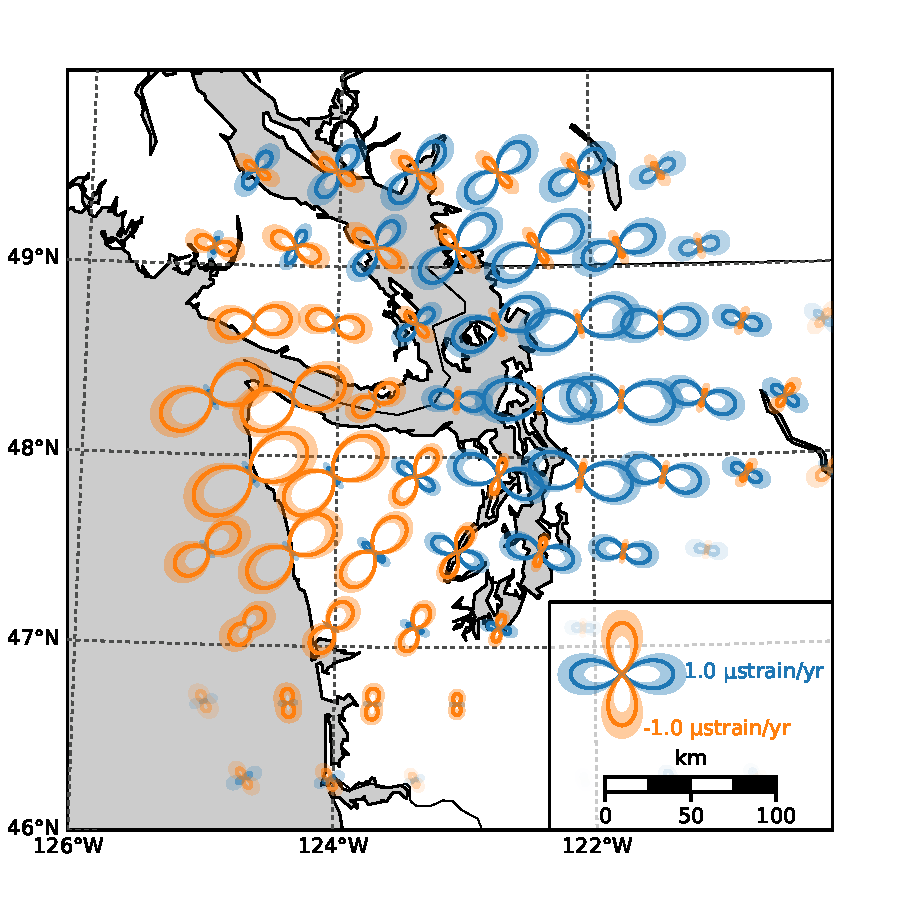
\includegraphics{figures/strain_map/strain-map.pdf}
\caption{Strain map.}   
\label{fig:Fit}
\end{figure*}

To demonstrate the effectiveness of our method for detecting SSEs, we show a timeseries of estimated strain components at the position indicated in figure X.  We also compare the strain rate magnitude and the frequency of tremors in this region.  The strain rate magnitudes have been normalized by its estimated uncertainty and so strain magnitudes less than ${\sim}$2 can be considered to be part of the background noise. The only time that the normalized strain rate magnitude exceeds 2 is when there is a corresponding peak in tremor.  We are able to accurately detect the seven SSEs in over this period in addition to the inter-SSE events such as the one at X.      

A video can be found as supp material 

made in ,  is accumulating to the trench perpendicular compression releases At the height of the SSE, the implications of    
  
model exhibits the same relationship  which can described  


Both of which have clear implications for assessing seismic hazard.

, which can have applications for seismic hazard assessment,Identifying strain resulting from ETS events serves two purposes: (1) ETS events have  events which are  were first discovered by \citet{Dragert2001}.   


We demonstrate that Gaussian processes are effective tools for detecting transient strain by using them to detect Cascadia slow slip events.  

BACKGROUND

\citet{Dragert2001} first discovered slow slip events

Explain strain concentration with this:

 
Interseismic locking depths from \citet{Fluck1997}, \citet{Murray2000}, \citet{McCaffrey2007} and \citet{McCaffrey2013}, \citet{Burgette2009}, \citet{schmalzle2014} are consistent with a full locking down to about 20 km.

%Studies which simultaneously looked at intersesimic and ets are \citet{Holtkamp2010} and \citet{Schmalzle2014}
Studies which simultaneously modeled interseismic and ets are \citet{Holtkamp2010} and \citet{schmalzle2014}


\section{Discussion and Conclusion}\label{sec:Discussion}
% discuss potential applications for slip models

% discuss how we remove errors like reference frame and seasonals

% discuss how this can be used for tikhonov regularization

% we do not interpolate the strain field because it may introduce spurious artifacts Baxter2011

% Discuss similarities with PCA used in Dong2006 and common mode error by Wdowinski1997
% note that these errors are due to long wavelength features which get removed in strain calculations!!!
% see strain method by almendinger2007

% mention the scec geodetic transient exercise Lohman2013 and references therein

% Note that segalls 2016 paper mentions the gap between interseismic and sse

% mention howell2016, who said some crap about verticals, mention Hammond2016 so said more sensible crap about verticals

% note that this can be used for smoothing verticals, and compare it with burgette2009

% change the notation for stencil size or smoothness order because they are both n. use p for smoothness order


The material presented in this paper is primarily focused on GPS data; however, we speculate that the RBF-FD scheme can be of particular use in denoising borehole strain meter (BSM) data.  The Plate Boundary Observatory has deployed X BSMs along the Western United States.  BSM data contains low frequency drift resulting from relaxation of the borehole \citep{Gladwin1987}, which can obscure the geophysical signal of interest.  We suggest that the RBF-FD scheme may be useful in denoising BSM data.  Since the RBF-FD scheme provides a straight-forward mapping from GPS displacements to strain at any target locations, it is possible to use GPS derived strains as \textit{a priori} information for strain at BSM sites. GPS derived strains could then aid in discerning tectonic signal from noise in BSM data.

Additional uses for strain: transient detection, prior for strain meters,  

Additional potential applications of the RBF-FD method: regularizing inverse problems, 

% cite eric calais for triangulation strain

\bibliographystyle{apalike}
\bibliography{mybib}  
 
\end{document}
